% !TeX program = xelatex
\documentclass[a4paper,10pt]{article}

% ============================================================================
% កញ្ចប់បណ្ណាល័យ (Packages) – តាមលំនាំ NGS Preah Krasang (ls_plan.tex)
% មេរៀនទី១៥ (ម៉ោងទី៣ / CIRC3)៖ ២.២ ធ្នូ និងអង្កត់ធ្នូ (ទំ.២០០–២០១)
% បរិបទ៖ គ្មានស្លាយ LCD — ប្រើក្ដារខៀន + សន្លឹកកិច្ចការ POE 1:1 & Backward-Faded Proof ជាគោល
% ============================================================================
\usepackage[a4paper, left=0.95cm, right=0.95cm, top=0.85cm, bottom=0.92cm, footskip=0.52cm]{geometry}
\usepackage{amsmath}
\usepackage{unicode-math}
\usepackage{fontspec}
\usepackage{array, longtable, multirow, colortbl}
\usepackage[table]{xcolor}
\usepackage{enumitem}
\usepackage{pifont}
\usepackage{fancyhdr}
\usepackage{tikz}
\usetikzlibrary{calc, arrows.meta, angles, quotes, decorations.markings, babel}

\makeatletter
\let\@expl@@@mark@update@singlecol@structures@@\relax
\makeatother

\providecommand{\NGSFindFonts}{%
  \IfFileExists{C:/Windows/Fonts/cambria.ttc}{%
    \def\NGSSysPath{C:/Windows/Fonts/}%
    \def\NGSUserPath{C:/Users/KIT/AppData/Local/Microsoft/Windows/Fonts/}%
  }{%
    \IfFileExists{./fonts/KhmerOSsiemreap.ttf}{\def\NGSSysPath{./fonts/}\def\NGSUserPath{./fonts/}}{%
    \IfFileExists{../fonts/KhmerOSsiemreap.ttf}{\def\NGSSysPath{../fonts/}\def\NGSUserPath{../fonts/}}{%
    \IfFileExists{../../fonts/KhmerOSsiemreap.ttf}{\def\NGSSysPath{../../fonts/}\def\NGSUserPath{../../fonts/}}{%
    \IfFileExists{../../../fonts/KhmerOSsiemreap.ttf}{\def\NGSSysPath{../../../fonts/}\def\NGSUserPath{../../../fonts/}}{%
    \IfFileExists{../../../../fonts/KhmerOSsiemreap.ttf}{\def\NGSSysPath{../../../../fonts/}\def\NGSUserPath{../../../../fonts/}}{%
    \IfFileExists{../../../../../fonts/KhmerOSsiemreap.ttf}{\def\NGSSysPath{../../../../../fonts/}\def\NGSUserPath{../../../../../fonts/}}{%
    \IfFileExists{../../../../../../fonts/KhmerOSsiemreap.ttf}{\def\NGSSysPath{../../../../../../fonts/}\def\NGSUserPath{../../../../../../fonts/}}{%
      \def\NGSSysPath{../../../../../../../fonts/}\def\NGSUserPath{../../../../../../../fonts/}%
    }}}}}}}%
  }%
}
\NGSFindFonts

\setmathfont[Path={\NGSSysPath}, FontIndex=1, Scale=1.02]{cambria.ttc}
\defaultfontfeatures{Ligatures=TeX}

\setmainfont[
  Path={\NGSUserPath}, Extension=.ttf, Script=Khmer,
  BoldFont={KhmerOSsiemreap}, BoldFeatures={FakeBold=1.8},
  ItalicFont={KhmerOSsiemreap}, ItalicFeatures={FakeSlant=0.25},
  BoldItalicFont={KhmerOSsiemreap}, BoldItalicFeatures={FakeBold=1.8, FakeSlant=0.25}
]{KhmerOSsiemreap}

\newfontfamily\muol[Path={\NGSUserPath}, Extension=.ttf, Script=Khmer]{KhmerOSmuollight}
\newfontfamily\TimesEn[Path={\NGSSysPath}, Extension=.ttf, BoldFont={timesbd}, ItalicFont={timesi}, BoldItalicFont={timesbi}]{times}
\newfontfamily\NagaBold[Path={\NGSUserPath}, Extension=.ttf]{AKbalthom Naga Bold}
\newfontfamily\CalibriFont[Path={\NGSSysPath}, Extension=.ttf]{calibri}
\newfontfamily\Tacteing[Path={\NGSUserPath}]{TACTENG.TTF}
\newfontfamily\CourierBullet[Path={\NGSSysPath}, Extension=.ttf]{cour}
\newcommand{\wcirc}{{\CourierBullet\fontsize{9.5pt}{11pt}\selectfont o}}

\XeTeXlinebreaklocale "km"
\XeTeXlinebreakskip = 0pt plus 1pt minus 0.1pt

\definecolor{stepgray}{HTML}{D9D9D9}
\definecolor{headgray}{HTML}{F2F2F2}
\definecolor{boxgray}{HTML}{D9D9D9}
\definecolor{darkred}{HTML}{C00000}
\definecolor{red5e}{HTML}{FF0000}

\pagestyle{fancy}
\fancyhf{}
\renewcommand{\headrulewidth}{0pt}
\fancyfoot[R]{\CalibriFont\fontsize{11pt}{13pt}\selectfont\thepage}

\setlength{\parindent}{0pt}
\setlength{\parskip}{0pt}
\setlength{\tabcolsep}{3.8pt}

\newcolumntype{L}[1]{>{\raggedright\arraybackslash}p{#1}}
\newcolumntype{C}[1]{>{\centering\arraybackslash}p{#1}}

\newcommand{\en}[1]{{\TimesEn #1}}
\newcommand{\enbf}[1]{{\TimesEn\textbf{#1}}}
\newcommand{\unit}[1]{\,\text{\en{#1}}}
\newcommand{\fiveE}[1]{{\NagaBold\fontsize{9.5pt}{13pt}\selectfont\textcolor{red5e}{#1}}}
\newcommand{\timenote}[1]{\textcolor{darkred}{\textit{#1}}}
\newcommand{\redsub}[1]{\textcolor{darkred}{#1}}
\newcommand{\graybox}[1]{\colorbox{boxgray}{\strut\hspace{2pt}#1\hspace{2pt}}}
\newcommand{\ditem}{\tikz[baseline=-0.5ex]\fill (0,0.42ex) -- (0.42ex,0) -- (0,-0.42ex) -- (-0.42ex,0) -- cycle;\hspace{0.3em}}
\newcommand{\cnum}[1]{{\fontsize{10.5pt}{12pt}\selectfont\ding{\numexpr181+#1\relax}}\hspace{0.2em}}
\newcommand{\cfig}[1]{\par\vspace{4pt}{\centering #1\par}\vspace{4pt}}
\newcommand{\stepheader}[1]{\multicolumn{3}{|c|}{\cellcolor{stepgray}\muol #1} \\* \noalign{\hrule height 0.4pt}}
\newcommand{\tri}[1]{\ensuremath{\triangle #1}}
\newcommand{\ang}[1]{\ensuremath{\angle #1}}
\newcommand{\arc}[1]{\ensuremath{\overset{\tikz[baseline=-0.55ex]\draw[black, line width=0.55pt] (0,0) to[bend left=40] (1.8ex,0);}{#1}}}
\newcommand{\khmflourish}{{\Tacteing\fontsize{36pt}{14pt}\selectfont\raisebox{-5pt}{3}}}

% -------------------- TikZ Helpers (B&W Print-Safe) --------------------
\newcommand{\tickmark}[3][1]{%
  \begin{scope}
    \coordinate (TMmid) at ($ (#2)!0.5!(#3) $);
    \pgfmathanglebetweenpoints{\pgfpointanchor{#2}{center}}{\pgfpointanchor{#3}{center}}
    \let\TMang\pgfmathresult
    \ifnum#1=1
      \draw[black, line width=0.75pt] ($(TMmid)+(\TMang+90:0.10)$) -- ($(TMmid)+(\TMang-90:0.10)$);
    \else
      \draw[black, line width=0.75pt] ($(TMmid)+(\TMang:0.04)+(\TMang+90:0.10)$) -- ($(TMmid)+(\TMang:0.04)+(\TMang-90:0.10)$);
      \draw[black, line width=0.75pt] ($(TMmid)+(\TMang:-0.04)+(\TMang+90:0.10)$) -- ($(TMmid)+(\TMang:-0.04)+(\TMang-90:0.10)$);
    \fi
  \end{scope}
}

% ============================================================================
% រូបធរណីមាត្រ TikZ ស-ខ្មៅ សម្រាប់ម៉ោងទី៣ (២.២ ធ្នូ និងអង្កត់ធ្នូ)
% ============================================================================

% ១. រំលឹកវិសមភាពត្រីកោណ និងលក្ខណៈត្រីកោណប៉ុនគ្នា (ជ.ជ.ជ)
\newcommand{\figPrereqCIRCThree}{%
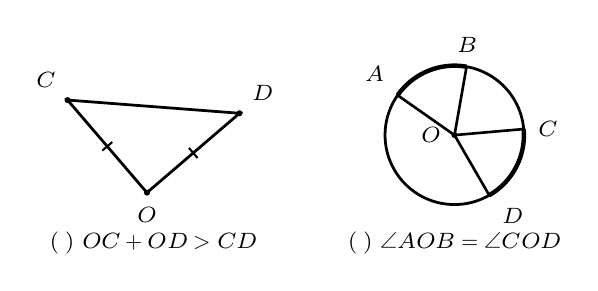
\begin{tikzpicture}[scale=0.84, every node/.style={font=\footnotesize, text=black}]
  % ខាងឆ្វេង៖ វិសមភាពត្រីកោណ OC + OD > CD
  \begin{scope}[shift={(0,0)}]
    \coordinate (O) at (1.35,0.28);
    \coordinate (C) at (0.15,1.68);
    \coordinate (D) at (2.75,1.48);
    \draw[black, line width=1.0pt] (O) -- (C) -- (D) -- cycle;
    \tickmark[1]{O}{C}
    \tickmark[1]{O}{D}
    \fill[black] (O) circle (1.3pt) node[below=1.5pt] {$O$};
    \fill[black] (C) circle (1.3pt) node[above left=1pt] {$C$};
    \fill[black] (D) circle (1.3pt) node[above right=1pt] {$D$};
    \node at (1.45,-0.48) {(ក) $OC+OD > CD$};
  \end{scope}
  % ខាងស្ដាំ៖ ធ្នូស្កាត់ដោយមុំផ្ចិតប៉ុនគ្នា
  \begin{scope}[shift={(4.60,0)}]
    \coordinate (O) at (1.40,1.15);
    \pgfmathsetmacro{\R}{1.05}
    \draw[black, line width=1.0pt] (O) circle (\R);
    \draw[black, line width=0.95pt] (O) -- ($(O)+(145:\R)$) node[above left=1pt] {$A$};
    \draw[black, line width=0.95pt] (O) -- ($(O)+(80:\R)$) node[above=1.5pt] {$B$};
    \draw[black, line width=0.95pt] (O) -- ($(O)+(5:\R)$) node[right=1.5pt] {$C$};
    \draw[black, line width=0.95pt] (O) -- ($(O)+(-60:\R)$) node[below right=1pt] {$D$};
    \draw[black, line width=1.6pt] ($(O)+(80:\R)$) arc (80:145:\R);
    \draw[black, line width=1.6pt] ($(O)+(-60:\R)$) arc (-60:5:\R);
    \fill[black] (O) circle (1.3pt) node[left=1.5pt] {$O$};
    \node at (1.40,-0.48) {(ខ) $\ang{AOB}=\ang{COD}$};
  \end{scope}
\end{tikzpicture}}

% ២. E1 Engage: បន្ទះឈើរាងរង្វង់មុខកាត់តុ (អង្កត់ធ្នូវែងបំផុត និងការទ្វេដងមុំ 60^\circ -> 120^\circ)
\newcommand{\figEngageCIRCThree}{%
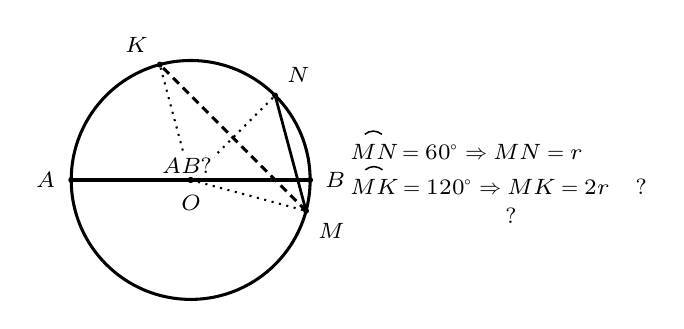
\begin{tikzpicture}[scale=0.82, every node/.style={font=\footnotesize, text=black}]
  \coordinate (O) at (0,0);
  \pgfmathsetmacro{\R}{1.85}
  \draw[black, line width=1.1pt] (O) circle (\R);
  \coordinate (P0) at (-15:\R);
  \coordinate (P1) at (45:\R);
  \coordinate (P2) at (105:\R);
  \coordinate (A) at (180:\R);
  \coordinate (B) at (0:\R);
  % អង្កត់ផ្ចិត AB និងអង្កត់ធ្នូ 60^\circ vs 120^\circ
  \draw[black, line width=1.15pt] (A) -- (B);
  \draw[black, line width=1.0pt] (P0) -- (P1);
  \draw[black, line width=1.05pt, densely dashed] (P0) -- (P2);
  \draw[black, line width=0.75pt, dotted] (O) -- (P0) (O) -- (P1) (O) -- (P2);
  \fill[black] (O) circle (1.4pt) node[below=2pt] {$O$};
  \fill[black] (A) circle (1.3pt) node[left=2pt] {$A$};
  \fill[black] (B) circle (1.3pt) node[right=2pt] {$B$};
  \fill[black] (P0) circle (1.3pt) node[below right=1pt] {$M$};
  \fill[black] (P1) circle (1.3pt) node[above right=1pt] {$N$};
  \fill[black] (P2) circle (1.3pt) node[above left=1pt] {$K$};
  \node[above=1pt, fill=white, inner sep=0.8pt] at (-0.45,0.02) {របារដែក $AB$?};
  \node[right=4pt] at (2.15,0.55) {$\arc{MN}=60^\circ \Rightarrow MN=r$};
  \node[right=4pt] at (2.15,0.00) {$\arc{MK}=120^\circ \Rightarrow MK = 2r$ ឬទេ?};
  \node[right=4pt] at (2.15,-0.55) {អង្កត់ធ្នូណាវែងជាងគេបំផុត?};
\end{tikzpicture}}

% ៣. E2 Explore & E3 Explain: ឧទាហរណ៍ទី១-២ និង ទ្រឹស្ដីបទ (ទំ.២០០-២០១)
\newcommand{\figTheoremCIRCThree}{%
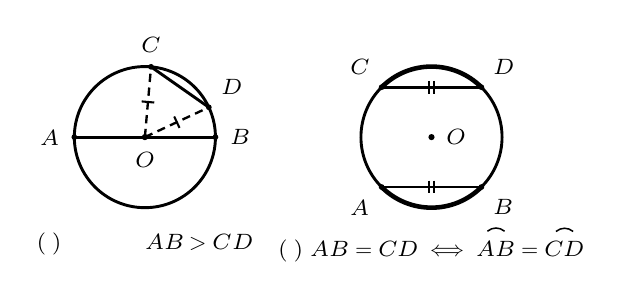
\begin{tikzpicture}[scale=0.80, every node/.style={font=\footnotesize, text=black}]
  % ខាងឆ្វេង៖ អង្កត់ផ្ចិត AB > អង្កត់ធ្នូ CD (លំហាត់គំរូទី១ ទំ.២០១)
  \begin{scope}[shift={(0,0)}]
    \coordinate (O) at (1.45,1.38);
    \pgfmathsetmacro{\R}{1.12}
    \coordinate (A) at ($(O)+(180:\R)$);
    \coordinate (B) at ($(O)+(0:\R)$);
    \coordinate (C) at ($(O)+(85:\R)$);
    \coordinate (D) at ($(O)+(25:\R)$);
    \draw[black, line width=1.05pt] (O) circle (\R);
    \draw[black, line width=1.15pt] (A) -- (B);
    \draw[black, line width=1.05pt] (C) -- (D);
    \draw[black, line width=0.85pt, densely dashed] (O) -- (C) (O) -- (D);
    \tickmark[1]{O}{C}
    \tickmark[1]{O}{D}
    \fill[black] (O) circle (1.4pt) node[below=2pt] {$O$};
    \fill[black] (A) circle (1.3pt) node[left=2pt] {$A$};
    \fill[black] (B) circle (1.3pt) node[right=2pt] {$B$};
    \fill[black] (C) circle (1.3pt) node[above=1.5pt] {$C$};
    \fill[black] (D) circle (1.3pt) node[above right=1pt] {$D$};
    \node at (1.45,-0.32) {(ក) អង្កត់ផ្ចិត $AB > CD$};
  \end{scope}
  % ខាងស្ដាំ៖ អង្កត់ធ្នូពីរប៉ុនគ្នា AB = CD <-> ធ្នូ AB = ធ្នូ CD
  \begin{scope}[shift={(4.55,0)}]
    \coordinate (O) at (1.45,1.38);
    \pgfmathsetmacro{\R}{1.12}
    \coordinate (A) at ($(O)+(-135:\R)$);
    \coordinate (B) at ($(O)+(-45:\R)$);
    \coordinate (C) at ($(O)+(135:\R)$);
    \coordinate (D) at ($(O)+(45:\R)$);
    \draw[black, line width=1.05pt] (O) circle (\R);
    \draw[black, line width=1.05pt] (A) -- (B);
    \draw[black, line width=1.05pt] (C) -- (D);
    \draw[black, line width=1.65pt] (A) arc (-135:-45:\R);
    \draw[black, line width=1.65pt] (D) arc (45:135:\R);
    \tickmark[2]{A}{B}
    \tickmark[2]{C}{D}
    \fill[black] (O) circle (1.4pt) node[right=2pt] {$O$};
    \fill[black] (A) circle (1.3pt) node[below left=1pt] {$A$};
    \fill[black] (B) circle (1.3pt) node[below right=1pt] {$B$};
    \fill[black] (C) circle (1.3pt) node[above left=1pt] {$C$};
    \fill[black] (D) circle (1.3pt) node[above right=1pt] {$D$};
    \node at (1.45,-0.32) {(ខ) $AB=CD \iff \arc{AB}=\arc{CD}$};
  \end{scope}
\end{tikzpicture}}

% ៤. E4 Elaborate: លំហាត់គំរូទី២ (MN=PQ) និង លំហាត់គំរូទី៣ (ធ្នូតូច AB > CD => AB > CD) (ទំ.២០១)
\newcommand{\figModelCIRCThree}{%
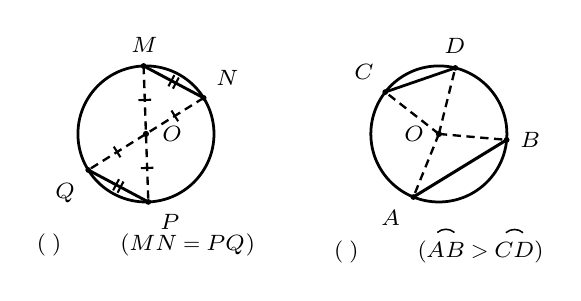
\begin{tikzpicture}[scale=0.80, every node/.style={font=\footnotesize, text=black}]
  % គំរូទី២៖ MN = PQ => \Delta NOM \cong \Delta POQ => \arc{MN} = \arc{PQ}
  \begin{scope}[shift={(0,0)}]
    \coordinate (O) at (1.45,1.45);
    \pgfmathsetmacro{\R}{1.08}
    \coordinate (M) at ($(O)+(92:\R)$);
    \coordinate (N) at ($(O)+(32:\R)$);
    \coordinate (P) at ($(O)+(-88:\R)$);
    \coordinate (Q) at ($(O)+(-148:\R)$);
    \draw[black, line width=1.0pt] (O) circle (\R);
    \draw[black, line width=1.05pt] (M) -- (N);
    \draw[black, line width=1.05pt] (P) -- (Q);
    \draw[black, line width=0.85pt, densely dashed] (M) -- (P) (N) -- (Q);
    \tickmark[1]{O}{M}
    \tickmark[1]{O}{N}
    \tickmark[1]{O}{P}
    \tickmark[1]{O}{Q}
    \tickmark[2]{M}{N}
    \tickmark[2]{P}{Q}
    \fill[black] (O) circle (1.4pt) node[right=2.5pt] {$O$};
    \fill[black] (M) circle (1.3pt) node[above=1.5pt] {$M$};
    \fill[black] (N) circle (1.3pt) node[above right=1pt] {$N$};
    \fill[black] (P) circle (1.3pt) node[below right=1pt] {$P$};
    \fill[black] (Q) circle (1.3pt) node[below left=1pt] {$Q$};
    \node at (1.45,-0.32) {(ក) គំរូទី២ ($MN=PQ$)};
  \end{scope}
  % គំរូទី៣៖ \arc{AB} > \arc{CD} => AB > CD
  \begin{scope}[shift={(4.65,0)}]
    \coordinate (O) at (1.45,1.45);
    \pgfmathsetmacro{\R}{1.08}
    \coordinate (A) at ($(O)+(-112:\R)$);
    \coordinate (B) at ($(O)+(-5:\R)$);
    \coordinate (C) at ($(O)+(142:\R)$);
    \coordinate (D) at ($(O)+(76:\R)$);
    \draw[black, line width=1.0pt] (O) circle (\R);
    \draw[black, line width=1.1pt] (A) -- (B);
    \draw[black, line width=1.0pt] (C) -- (D);
    \draw[black, line width=0.85pt, densely dashed] (O) -- (A) (O) -- (B) (O) -- (C) (O) -- (D);
    \fill[black] (O) circle (1.4pt) node[left=2pt] {$O$};
    \fill[black] (A) circle (1.3pt) node[below left=1pt] {$A$};
    \fill[black] (B) circle (1.3pt) node[right=1.5pt] {$B$};
    \fill[black] (C) circle (1.3pt) node[above left=1pt] {$C$};
    \fill[black] (D) circle (1.3pt) node[above=1.5pt] {$D$};
    \node at (1.45,-0.32) {(ខ) គំរូទី៣ ($\arc{AB}>\arc{CD}$)};
  \end{scope}
\end{tikzpicture}}

% ៥. E5 Evaluate (លំហាត់ទី២ ទំ.២០៤៖ \arc{AD} = \arc{CB} => AC = BD)
\newcommand{\figPracticeCIRCThree}{%
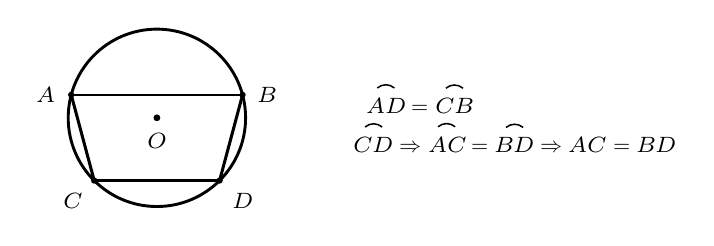
\begin{tikzpicture}[scale=0.88, every node/.style={font=\footnotesize, text=black}]
  \coordinate (O) at (0,0);
  \pgfmathsetmacro{\R}{1.28}
  \coordinate (A) at (165:\R);
  \coordinate (B) at (15:\R);
  \coordinate (C) at (-135:\R);
  \coordinate (D) at (-45:\R);
  \draw[black, line width=1.05pt] (O) circle (\R);
  \draw[black, line width=0.85pt] (A) -- (B) (C) -- (D);
  \draw[black, line width=1.1pt] (A) -- (C) (B) -- (D);
  \fill[black] (O) circle (1.4pt) node[below=2pt] {$O$};
  \fill[black] (A) circle (1.3pt) node[left=2pt] {$A$};
  \fill[black] (B) circle (1.3pt) node[right=2pt] {$B$};
  \fill[black] (C) circle (1.3pt) node[below left=1pt] {$C$};
  \fill[black] (D) circle (1.3pt) node[below right=1pt] {$D$};
  \node[right=4pt] at (1.62,0.28) {សម្មតិកម្ម៖ $\arc{AD}=\arc{CB}$};
  \node[right=4pt] at (1.62,-0.28) {ដកធ្នូរួម $\arc{CD} \Rightarrow \arc{AC}=\arc{BD} \Rightarrow AC=BD$};
\end{tikzpicture}}

% ៦. កិច្ចការផ្ទះ៖ លំហាត់ទី៣ និង ទី៥ (ទំ.២០៤)
\newcommand{\figHWCIRCThree}{%
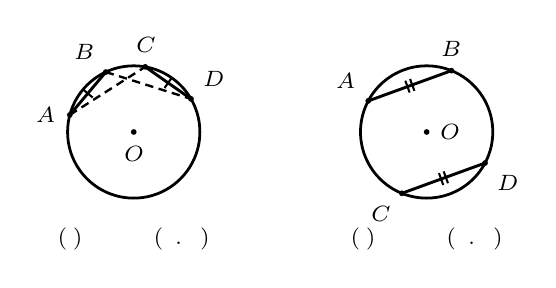
\begin{tikzpicture}[scale=0.80, every node/.style={font=\footnotesize, text=black}]
  % លំហាត់ទី៣៖ AB = CD => \arc{AC} = \arc{BD}
  \begin{scope}[shift={(0,0)}]
    \coordinate (O) at (1.45,1.38);
    \pgfmathsetmacro{\R}{1.05}
    \coordinate (A) at ($(O)+(165:\R)$);
    \coordinate (B) at ($(O)+(115:\R)$);
    \coordinate (C) at ($(O)+(80:\R)$);
    \coordinate (D) at ($(O)+(30:\R)$);
    \draw[black, line width=1.0pt] (O) circle (\R);
    \draw[black, line width=1.05pt] (A) -- (B) (C) -- (D);
    \draw[black, line width=0.85pt, densely dashed] (A) -- (C) (B) -- (D);
    \tickmark[1]{A}{B}
    \tickmark[1]{C}{D}
    \fill[black] (O) circle (1.3pt) node[below=1.5pt] {$O$};
    \fill[black] (A) circle (1.3pt) node[left=1.5pt] {$A$};
    \fill[black] (B) circle (1.3pt) node[above left=1pt] {$B$};
    \fill[black] (C) circle (1.3pt) node[above=1.5pt] {$C$};
    \fill[black] (D) circle (1.3pt) node[above right=1pt] {$D$};
    \node at (1.45,-0.32) {(ក) លំហាត់ទី៣ (ទំ.២០៤)};
  \end{scope}
  % លំហាត់ទី៥៖ AB = CD => \arc{BD} = \arc{AC}
  \begin{scope}[shift={(4.65,0)}]
    \coordinate (O) at (1.45,1.38);
    \pgfmathsetmacro{\R}{1.05}
    \coordinate (A) at ($(O)+(152:\R)$);
    \coordinate (B) at ($(O)+(68:\R)$);
    \coordinate (D) at ($(O)+(-28:\R)$);
    \coordinate (C) at ($(O)+(-112:\R)$);
    \draw[black, line width=1.0pt] (O) circle (\R);
    \draw[black, line width=1.05pt] (A) -- (B) (C) -- (D);
    \tickmark[2]{A}{B}
    \tickmark[2]{C}{D}
    \fill[black] (O) circle (1.3pt) node[right=1.5pt] {$O$};
    \fill[black] (A) circle (1.3pt) node[above left=1pt] {$A$};
    \fill[black] (B) circle (1.3pt) node[above=1.5pt] {$B$};
    \fill[black] (D) circle (1.3pt) node[below right=1pt] {$D$};
    \fill[black] (C) circle (1.3pt) node[below left=1pt] {$C$};
    \node at (1.45,-0.32) {(ខ) លំហាត់ទី៥ (ទំ.២០៤)};
  \end{scope}
\end{tikzpicture}}

% ============================================================================
% ចាប់ផ្ដើមឯកសារ (Document Body)
% ============================================================================
\begin{document}
\fontsize{10pt}{15.2pt}\selectfont

% -------------------- ក្បាលកិច្ចតែងការ (Header) --------------------
\begin{center}
  {\muol\fontsize{11pt}{16pt}\selectfont ព្រះរាជាណាចក្រកម្ពុជា}\\[2pt]
  {\muol\fontsize{10pt}{15pt}\selectfont ជាតិ សាសនា ព្រះមហាក្សត្រ}\\[1pt]
  \khmflourish
\end{center}

\vspace{-28pt}
{\muol\fontsize{9.5pt}{12.5pt}\selectfont
មន្ទីរអប់រំ យុវជន និងកីឡា ខេត្តកំពង់ធំ\\
ការិយាល័យអប់រំ យុវជន និងកីឡា ស្រុកកំពង់ស្វាយ\\
អនុវិទ្យាល័យព្រះក្រសាំង}

\vspace{1pt}
\begin{center}
  {\muol\fontsize{10pt}{14pt}\selectfont កិច្ចតែងការបង្រៀន}
\end{center}
\vspace{0pt}

% -------------------- ព័ត៌មានទូទៅ (Metadata) --------------------
{\renewcommand{\arraystretch}{0.95}
\hspace*{4.05cm}%
\begin{tabular}{@{}l l l@{}}
  - \hspace{0.35cm} មុខវិជ្ជា & : & គណិតវិទ្យា ថ្នាក់ទី៨ \\
  - \hspace{0.35cm} ចំណងជើងមេរៀន & : & មេរៀនទី១៥ រង្វង់ \\
  - \hspace{0.35cm} ចំណងជើងរង & : & ២.២ ធ្នូ និងអង្កត់ធ្នូ (ទំ.២០០--២០១) \\
  - \hspace{0.35cm} រយៈពេល & : & ១ ម៉ោងសិក្សា (៥០ នាទី) \\
  - \hspace{0.35cm} បង្រៀនដោយ & : & ហុក ប៊ុនថែន \\
  - \hspace{0.35cm} កាលបរិច្ឆេទ & : & ថ្ងៃពុធ ទី១៦ ខែធ្នូ ឆ្នាំ២០២៦ \\
\end{tabular}

\vspace{1pt}

% -------------------- I. វត្ថុបំណង --------------------
\textbf{I.} {\muol វត្ថុបំណង}\\[1pt]
\hspace*{0.55cm}%
\begin{tabular}{@{}l l L{14.2cm}@{}}
  \wcirc \hspace{0.25cm} វិជ្ជាសម្បទា & : & សិស្សប្រាប់និយមន័យនិងនិមិត្តសញ្ញាសម្គាល់ធ្នូ ($\arc{AB}$) និងអង្កត់ធ្នូ ($AB$) ព្រមទាំងពោលទ្រឹស្ដីបទអង្កត់ផ្ចិតជាអង្កត់ធ្នូវែងជាងគេ និងទ្រឹស្ដីបទសមមូលរវាងធ្នូប៉ុនគ្នានិងអង្កត់ធ្នូប៉ុនគ្នាបានត្រឹមត្រូវ ។ \\
  \wcirc \hspace{0.25cm} បំណិនសម្បទា & : & សិស្សវាស់ប្រៀបធៀបប្រវែងអង្កត់ធ្នូលើសន្លឹកកិច្ចការ និងស្រាយបញ្ជាក់ទំនាក់ទំនងរវាងធ្នូនិងអង្កត់ធ្នូតាមវិសមភាពត្រីកោណ ត្រីកោណប៉ុនគ្នា និងការបូក-ដកធ្នូរួមបានត្រឹមត្រូវ ។ \\
  \wcirc \hspace{0.25cm} ចរិយាសម្បទា & : & សិស្សមានទម្លាប់ផ្ទៀងផ្ទាត់ការទស្សន៍ទាយដោយរង្វាស់ជាក់ស្ដែង សរសេរហេតុផលធរណីមាត្រមានលំដាប់លំដោយ និងសហការពិភាក្សាក្នុងក្រុមដោយស្មារតីទទួលខុសត្រូវ ។ \\
\end{tabular}

\vspace{1pt}

% -------------------- II. សម្ភារៈឧបទេស --------------------
\textbf{II.} {\muol សម្ភារៈឧបទេស}\\[1pt]
\hspace*{0.55cm}$\bullet$ \hspace{0.35cm} សៀវភៅសិក្សាគោលថ្នាក់ទី៨ (ទំ.២០០--២០១, ២០៤) ក្ដារខៀន ដីស បន្ទាត់ក្រិត ដែកឈានក្ដារខៀន ព្រមទាំង\textbf{សន្លឹកកិច្ចការសិស្ស ស-ខ្មៅ (\en{Worksheet\_CIRC3} ទំព័រ ១--២)} (បង្រៀនដោយគ្មានស្លាយ \en{LCD})

\vspace{1pt}

% -------------------- III. វិធីសាស្រ្តបង្រៀន --------------------
\textbf{III.} {\muol វិធីសាស្រ្តបង្រៀន}\\[1pt]
\hspace*{0.45cm}%
\begin{tabular}{@{}l l L{14.85cm}@{}}
  $\bullet$ \hspace{0.25cm} គោលវិធី & : & សិស្សមជ្ឈមណ្ឌល (ប្រើសន្លឹកកិច្ចការពិសោធន៍ និងបំពេញសម្រាយបញ្ជាក់ ស-ខ្មៅ ជាគោល គ្មានស្លាយ \en{LCD}) \\
  $\bullet$ \hspace{0.25cm} យុទ្ធវិធីបង្រៀន & : & គំរូ 5Es រួមផ្សំ \en{POE} (ទស្សន៍ទាយ--វាស់ផ្ទៀង--ពន្យល់លើរូបខ្នាតពិត 1:1) និងសម្រាយបញ្ជាក់បន្ថយជំនួយជាជំហាន (\en{Backward-Faded Proof}) ភ្ជាប់ធនាគារហេតុផល \cnum{1}--\cnum{5} \\
\end{tabular}
}

\vspace{1pt}

% -------------------- IV. ដំណើរការបង្រៀន --------------------
\textbf{IV.} {\muol ដំណើរការបង្រៀន}

\vspace{1pt}

\renewcommand{\arraystretch}{1.15}
\begin{longtable}{|L{5.50cm}|L{7.90cm}|L{4.80cm}|}
\hline
\rowcolor{headgray}
\multicolumn{1}{|c|}{\muol សកម្មភាពគ្រូ} &
\multicolumn{1}{c|}{\muol ខ្លឹមសារមេរៀន} &
\multicolumn{1}{c|}{\muol សកម្មភាពសិស្ស} \\
\hline
\endfirsthead

\hline
\endhead

\hline
\endfoot

\hline
\endlastfoot

% ==================== ជំហានទី១ (2min) ====================
\stepheader{ជំហានទី១ \enbf{(}រដ្ឋបាលថ្នាក់\enbf{)}}
$\bullet$ ពិនិត្យអវត្តមាន សណ្ដាប់ធ្នាប់ អនាម័យ និងការត្រៀមបន្ទាត់ក្រិតមីលីម៉ែត្រ ដែកឈាន
&
$\bullet$ រដ្ឋបាលថ្នាក់ និងការត្រៀមបន្ទាត់ក្រិតវាស់អង្កត់ធ្នូលើសន្លឹកកិច្ចការ
&
$\circ$ ប្រធានថ្នាក់រាយការណ៍អវត្តមាន និងត្រៀមបន្ទាត់ក្រិត \\[3pt]

$\bullet$ ចែក \textbf{សន្លឹកកិច្ចការ ១៥.៣} (ទំព័រ ១--២) ជូនសិស្សគ្រប់គ្នាផ្កាប់ទុកលើតុ
&
$\bullet$ សន្លឹកកិច្ចការ \en{POE} និងសម្រាយបញ្ជាក់បន្ថយជំនួយ (\en{Backward-Faded Proof})
&
$\circ$ ទទួលសន្លឹកកិច្ចការផ្កាប់លើតុ រង់ចាំការណែនាំ \\
\hline

% ==================== ជំហានទី២ (9min: <=3 + 3 + E1 3) ====================
\stepheader{ជំហានទី២ \enbf{(}ពិនិត្យចំណេះដឹងមុន \enbf{+} ទំនាក់ទំនងមេរៀនថ្មី\enbf{)}}
\ditem \textbf{ពិនិត្យកិច្ចការផ្ទះ ($\le 3\unit{min}$)} \timenote{ផ្ទៀងចម្លើយខ្លីលើក្ដារ} \par
$\bullet$ ហៅសិស្ស ២ នាក់ឆ្លើយផ្ទាល់មាត់ពីលទ្ធផលលំហាត់ទី១ (ទំ.២០៤) និងប្រវែងធ្នូនៅកាំ $r=18\unit{cm}$
&
{\centering\redsub{កំណែកិច្ចការផ្ទះ (លំហាត់ទី១ ទំ.២០៤)}\par} \par
$\bullet$ \textbf{១. រង្វាស់ដឺក្រេធ្នូតូច៖} $OA=OB=r \Rightarrow \ang{OBA}=\ang{OAB}=25^\circ \Rightarrow \ang{AOB}=180^\circ-50^\circ=130^\circ \Rightarrow \text{m}\arc{AB} = \graybox{$130^\circ$}$ ។ \par
$\bullet$ \textbf{២. ប្រវែងធ្នូ៖} $l = \frac{2\times 3.14 \times 18 \times 130^\circ}{360^\circ} = 40.82\unit{cm}$ ។
&
$\circ$ ផ្ទៀងផ្ទាត់ចម្លើយកិច្ចការផ្ទះក្នុងសៀវភៅរៀងៗខ្លួន \\[3pt]

\ditem \textbf{រំលឹកមេរៀនទាក់ទង (3min)} \timenote{សរុបកុំឱ្យលើស 3min} \par
$\bullet$ សួរសំណួររំលឹកវិសមភាពត្រីកោណ និងទំនាក់ទំនងរវាងមុំផ្ចិតប៉ុនគ្នានិងធ្នូស្កាត់
&
{\centering\redsub{រំលឹកវិសមភាពត្រីកោណ និងលក្ខណៈមុំផ្ចិត--ធ្នូ}\par} \par
$\bullet$ ក្នុង $\tri{OCD}$៖ ផលបូករង្វាស់ជ្រុងពីរធំជាងជ្រុងទីបី ($OC + OD > CD$) ។ \par
$\bullet$ ក្នុង $C(O,r)$៖ $\ang{AOB} = \ang{COD} \iff \arc{AB} = \arc{CD}$ ។
&
$\circ$ ឆ្លើយផ្ទាល់មាត់៖ «$OC+OD > CD$ ហើយមុំផ្ចិតប៉ុនគ្នាស្កាត់ធ្នូប៉ុនគ្នា!» \\[3pt]

&
\cfig{\figPrereqCIRCThree}
& \\[3pt]

\fiveE{E1 - Engage (3min)} \timenote{(បំផុសចម្ងល់ — កុំទាន់ផ្ដល់ចម្លើយ)} \par
\ditem \textbf{បញ្ហាជីវភាពពិត (ជាងឈើដាក់របារដែកទ្រមុខតុមូល)៖} \par
ជាងឈើត្រូវដាក់របារដែកត្រង់មួយកាត់មុខតុមូល $C(O,r)$ ឱ្យបានវែងបំផុត និងកាត់ក្បាច់គែមត្រង់ពីរ
&
{\centering\redsub{បេសកកម្មជាងឈើ៖ មុំទ្វេដង តើអង្កត់ធ្នូទ្វេដងដែរឬទេ?}\par}
&
$\circ$ សង្កេតរូបមុខតុមូលលើក្ដារខៀន និងអានបេសកកម្មលើសន្លឹកកិច្ចការ \\[3pt]

&
\cfig{\figEngageCIRCThree}
& \\[3pt]

– \textbf{សំណួរបំផុស៖} (១) តើរបារដែកត្រង់ត្រូវដាក់តាមទីតាំងណាទើបវែងជាងគេបំផុត? (២) បើធ្នូកើនពី $60^\circ$ ទៅ $120^\circ$ តើអង្កត់ធ្នូកើនទ្វេដង ($2r$) ដែរឬទេ?
&
\textbf{ចម្ងល់គោល៖} \par
$\bullet$ តើហេតុអ្វីអង្កត់ផ្ចិតជាអង្កត់ធ្នូវែងជាងគេក្នុងរង្វង់? \par
$\bullet$ តើធ្នូប៉ុនគ្នា និងធ្នូតូចមិនប៉ុនគ្នា ទាក់ទងនឹងប្រវែងអង្កត់ធ្នូយ៉ាងដូចម្ដេច?
&
$\circ$ ទស្សន៍ទាយក្នុងក្រុម និងកត់ចម្លើយទាយលើសន្លឹកកិច្ចការ (ផ្នែក ក) \\
\hline

% ==================== ជំហានទី៣ (17min: E2 11m + E3 6m) ====================
\stepheader{ជំហានទី៣ \enbf{(}ខ្លឹមសារមេរៀនថ្មី\enbf{)}}
\fiveE{E2 - Explore (11min)} \par
$\bullet$ សរសេរចំណងជើងមេរៀនរងលើក្ដារខៀន និងណែនាំនិមិត្តសញ្ញាសម្គាល់ធ្នូ $\arc{AB}$ និងអង្កត់ធ្នូ $AB$ (ទំ.២០០)
&
២.២ ធ្នូ និងអង្កត់ធ្នូ (ទំ.២០០--២០១) \par
$\bullet$ \textbf{កំណត់សរសេរ៖} គេកំណត់ធ្នូដោយ $\arc{AB}$ (ខ្សែកោងលើរង្វង់) និងអង្កត់ធ្នូដោយ $AB$ (អង្កត់ត្រង់ភ្ជាប់ $A,B$) ។
&
$\circ$ កត់ចំណងជើង និងបែងចែកនិមិត្តសញ្ញា $\arc{AB}$ និង $AB$ \\[3pt]

\ditem \textbf{ពិសោធន៍ POE លើសន្លឹកកិច្ចការទំព័រ ១ (ផ្នែក ក — 6min)៖} \par
$\bullet$ ឱ្យសិស្សប្រើបន្ទាត់ក្រិតវាស់អង្កត់ធ្នូលើរង្វង់ខ្នាតពិត $C(O, 2.20\unit{cm})$ សម្រាប់មុំផ្ចិត $60^\circ, 60^\circ, 120^\circ, 180^\circ$ និងធ្នូធំ $240^\circ$
&
{\centering\textbf{លទ្ធផលវាស់ផ្ទាល់លើរង្វង់ខ្នាតពិត $r = 2.20\unit{cm}$}\par} \par
$\bullet$ ធ្នូ $60^\circ$ ពីរ ($\arc{EF}=\arc{GH}=60^\circ$) $\Rightarrow EF = GH = 2.20\unit{cm}$ (ប៉ុនគ្នា!) ។ \par
$\bullet$ ធ្នូ $120^\circ$ ($\arc{MK}$) $\Rightarrow MK \approx 3.81\unit{cm} \ne 4.40\unit{cm}$ (\textbf{មិនកើនទ្វេដងទេ!}) ។
&
$\circ$ ប្រើបន្ទាត់វាស់ប្រវែងអង្កត់ធ្នូទាំង ៥ បំពេញក្នុងតារាង \en{POE} \\[3pt]

– \textbf{អន្ទាក់ការយល់ច្រឡំ (Misconception Trap)៖} ចុះធ្នូធំ $240^\circ$ វែងជាងកន្លះរង្វង់ $180^\circ$ តើអង្កត់ធ្នូរបស់វាវែងជាងអង្កត់ផ្ចិតឬទេ?
&
$\bullet$ អង្កត់ផ្ចិត ($180^\circ$) $\Rightarrow AB = 2r = 4.40\unit{cm}$ (\textbf{វែងជាងគេបំផុត!}) ។ \par
$\bullet$ ធ្នូធំ $240^\circ$ មានអង្កត់ធ្នូត្រឹម $3.81\unit{cm} < 4.40\unit{cm}$ $\Rightarrow$ ការប្រៀបធៀបធ្នូវែងជាងឱ្យអង្កត់ធ្នូវែងជាង ពិត\textbf{ចំពោះតែធ្នូតូច ($<180^\circ$)} ប៉ុណ្ណោះ!
&
$\circ$ រកឃើញថាអង្កត់ផ្ចិត $4.40\unit{cm}$ វែងជាងគេ ហើយធ្នូធំ $240^\circ$ មានអង្កត់ធ្នូខ្លីជាងអង្កត់ផ្ចិត! \\[3pt]

\ditem \textbf{សកម្មភាពភ្ជាប់ឧទាហរណ៍ទី១ និងទី២ (ទំ.២០០ — 5min)៖} \par
$\bullet$ ឱ្យសិស្សពិនិត្យការត្រួតស៊ីគ្នានៃធ្នូប៉ុនគ្នា និងចុងធ្នូក្នុងឧទាហរណ៍ទី១--២ លើសន្លឹកកិច្ចការ
&
$\bullet$ \textbf{ឧទាហរណ៍ទី១៖} បើ $\arc{AB} = \arc{MN}$ (ត្រួតស៊ីគ្នា) នោះអង្កត់ធ្នូ $AB$ ត្រួតលើ $MN \Rightarrow AB = MN$ ។ \par
$\bullet$ \textbf{ឧទាហរណ៍ទី២៖} ច្រាសមកវិញ បើអង្កត់ធ្នូ $AB = CD$ នោះចុងធ្នូត្រួតស៊ីគ្នា $\Rightarrow \arc{AB} = \arc{CD}$ ។
&
$\circ$ គូសសញ្ញាឆ្នូតស្មើគ្នា (\textbf{[tracing]}) លើអង្កត់ធ្នូ និងធ្នូប៉ុនគ្នា \\[3pt]

% --- E3 Explain (6min) ---
\fiveE{E3 - Explain (6min)} \par
\ditem \textbf{សំយោគទ្រឹស្ដីបទ (ទំ.២០១) និងធនាគារហេតុផល \cnum{1}--\cnum{5}} \par
$\bullet$ ឱ្យតំណាងក្រុមឡើងបង្ហាញការរកឃើញ រួចគ្រូសង្ខេបទ្រឹស្ដីបទទាំងអស់លើក្ដារខៀន
&
{\muol ទ្រឹស្ដីបទ} \textbf{(ទំ.២០១)៖} \par
១. \textbf{អង្កត់ផ្ចិតជាអង្កត់ធ្នូដែលវែងជាងគេ}នៅក្នុងរង្វង់មួយ ($AB > CD$) ។ \par
២. ក្នុងរង្វង់មួយ ឬរង្វង់ពីរប៉ុនគ្នា៖ \textbf{បើធ្នូប៉ុនគ្នា នោះអង្កត់ធ្នូសន្ធឹងធ្នូទាំងពីរក៏ប៉ុនគ្នាដែរ} ហើយច្រាសមកវិញ \textbf{បើអង្កត់ធ្នូពីរប៉ុនគ្នា នោះធ្នូសន្ធឹងក្រោមអង្កត់ធ្នូទាំងពីរក៏ប៉ុនគ្នាដែរ} ($\arc{AB}=\arc{CD} \iff AB=CD$) ។
&
$\circ$ បំពេញប្រអប់ទ្រឹស្ដីបទក្នុងផ្នែក ខ នៃសន្លឹកកិច្ចការទំព័រ ១ \\[3pt]

&
\cfig{\figTheoremCIRCThree}
& \\[3pt]

$\bullet$ បន្ថែមវិបាកប្រៀបធៀបធ្នូតូចមិនប៉ុនគ្នា និងសង្ខេប\textbf{ធនាគារហេតុផល \cnum{1}--\cnum{5}} សម្រាប់សរសេរសម្រាយបញ្ជាក់
&
$\bullet$ \textbf{ប្រៀបធៀបធ្នូតូច៖} ក្នុង $C(O,r)$ ចំពោះធ្នូតូចពីរ៖ $\arc{AB} > \arc{CD} \iff AB > CD$ ។ \par
\textbf{ធនាគារហេតុផល៖} \cnum{1} កាំរង្វង់តែមួយស្មើគ្នា \textbar{} \cnum{2} វិសមភាពត្រីកោណ ($OC+OD>CD$) \textbar{} \cnum{3} ត្រីកោណប៉ុនគ្នា (ជ.ជ.ជ) \textbar{} \cnum{4} សមមូលធ្នូ--អង្កត់ធ្នូ ($\arc{AB}=\arc{CD}\iff AB=CD$) \textbar{} \cnum{5} វិសមភាពធ្នូតូច ($\arc{AB}>\arc{CD}\iff AB>CD$) ។
&
$\circ$ កត់ត្រាលេខកូដហេតុផល \cnum{1}--\cnum{5} សម្រាប់ប្រើក្នុងផ្នែក គ--ឃ \\
\hline

% ==================== ជំហានទី៤ (20min: E4 10m + E5 10m) ====================
\stepheader{ជំហានទី៤ \enbf{(}ពង្រីកចំណេះដឹង\enbf{)}}
\fiveE{E4 - Elaborate (10min)} \par
\ditem \textbf{សម្រាយបញ្ជាក់បន្ថយជំនួយ (Backward-Faded Proof) — លំហាត់គំរូទី១, ទី២ និងទី៣ (ទំ.២០១)} \par
$\bullet$ \textbf{ជំហានបន្ថយជំនួយទី១ (គំរូទី១ — 3min)៖} ដឹកនាំសិស្សបំពេញសេចក្ដីសន្និដ្ឋានចុងក្រោយនៃសម្រាយបញ្ជាក់ $AB > CD$
&
{\muol លំហាត់គំរូទី១} \textbf{(ទំ.២០១)៖} អង្កត់ផ្ចិត $AB$ និងអង្កត់ធ្នូ $CD$ (មិនកាត់ $O$) ។ បង្ហាញថា $AB > CD$ ។ \par
$\bullet$ ភ្ជាប់ $OC, OD$ ៖ ក្នុង $\tri{CDO}$ មាន $OC + OD > CD$ $(i)$ តាម \cnum{2} ។ \par
$\bullet$ តែ $OC + OD = r + r = AB$ $(ii)$ តាម \cnum{1} $\Rightarrow$ តាម $(i)$ និង $(ii)$ បាន \graybox{$AB > CD$} ។
&
$\circ$ គូសបន្ទាត់ជំនួយដាច់ៗ $OC, OD$ និងបំពេញចន្លោះគំរូទី១ លើសន្លឹកកិច្ចការទំព័រ ២ \\[3pt]

$\bullet$ \textbf{ជំហានបន្ថយជំនួយទី២ (គំរូទី២ — 3.5min)៖} ឱ្យសិស្សបំពេញហេតុផល និងវិបាកនៃសម្រាយបញ្ជាក់ $MN=PQ \Rightarrow \arc{MN}=\arc{PQ}$
&
{\muol លំហាត់គំរូទី២} \textbf{(ទំ.២០១)៖} ក្នុងរង្វង់ផ្ចិត $O$ មានអង្កត់ធ្នូ $MN = PQ$ ។ ស្រាយថា $\arc{MN} = \arc{PQ}$ ។ \par
$\bullet$ ក្នុង $\tri{NOM}$ និង $\tri{POQ}$ មាន៖ $OM=OP=r$, $ON=OQ=r$ (\cnum{1}) និង $MN=PQ$ (សម្មតិកម្ម) ។ \par
$\bullet$ នាំឱ្យ $\tri{NOM} \cong \tri{POQ}$ តាមករណីទី៣ (ជ.ជ.ជ \cnum{3}) $\Rightarrow \ang{NOM} = \ang{POQ} \Rightarrow \graybox{$\arc{MN} = \arc{PQ}$}$ ។
&
$\circ$ គូសសញ្ញាឆ្នូតស្មើគ្នាលើកាំ និងអង្កត់ធ្នូ រួចបំពេញជំហានបន្ថយជំនួយទី២ \\[3pt]

&
\cfig{\figModelCIRCThree}
& \\[3pt]

$\bullet$ \textbf{ជំហានបន្ថយជំនួយទី៣ (គំរូទី៣ — 3.5min)៖} ឱ្យសិស្សសរសេរជំហានប្រៀបធៀប $\arc{AB} > \arc{CD} \Rightarrow AB > CD$ និងឆ្លើយសំណួរ EIA 30s
&
{\muol លំហាត់គំរូទី៣} \textbf{(ទំ.២០១)៖} ក្នុង $C(O,r)$ មានធ្នូតូច $\arc{AB} > \arc{CD}$ ។ ស្រាយថា $AB > CD$ ។ \par
$\bullet$ ក្នុង $\tri{AOB}$ និង $\tri{COD}$ មាន $OA=OC=OB=OD=r$ (\cnum{1}) តែដោយ $\arc{AB} > \arc{CD}$ នោះមុំផ្ចិតចន្លោះជ្រុងស្មើគ្នាផ្ទៀងផ្ទាត់ $\ang{AOB} > \ang{COD} \Rightarrow \graybox{$AB > CD$}$ ។ \par
\timenote{EIA 30s៖ ហេតុអ្វីត្រូវបញ្ជាក់ពាក្យ «ធ្នូតូច»? (ព្រោះបើធ្នូធំ $>180^\circ$ ធ្នូកាន់តែវែង អង្កត់ធ្នូបែរជាកាន់តែខ្លី!)}
&
$\circ$ សរសេរសម្រាយបញ្ជាក់គំរូទី៣ និងឆ្លើយសំណួរ EIA 30s ផ្ទាល់មាត់ \\[3pt]

\fiveE{E5 - Evaluate (10min)} \par
\ditem \textbf{សម្រាយបញ្ជាក់ដោយខ្លួនឯង៖ លំហាត់ទី២ (ទំ.២០៤ — 6.5min ផ្នែក ឃ)} \par
$\bullet$ ឱ្យសិស្សស្រាយបញ្ជាក់ \textbf{លំហាត់ទី២ (ទំ.២០៤)} ដោយប្រើវិធីដកធ្នូរួម $\arc{CD}$ និងទ្រឹស្ដីបទសមមូល \cnum{4}
&
{\muol លំហាត់អនុវត្ត} \textbf{(លំហាត់ទី២ ទំ.២០៤)៖} ក្នុង $C(O,r)$ គេមាន $\arc{AD} = \arc{CB}$ ។ ស្រាយបញ្ជាក់ថា $AC = BD$ ។ \par
$\bullet$ គេមាន៖ $\arc{AD} = \arc{AC} + \arc{CD}$ និង $\arc{CB} = \arc{BD} + \arc{CD}$ ។ \par
$\bullet$ ដោយ $\arc{AD} = \arc{CB}$ (សម្មតិកម្ម) ដកធ្នូរួម $\arc{CD}$ ពីអង្គទាំងពីរ បាន $\arc{AC} = \arc{BD}$ ។ \par
$\bullet$ តាមទ្រឹស្ដីបទ \cnum{4} ($\arc{AC}=\arc{BD}$) នាំឱ្យអង្កត់ធ្នូ \graybox{$AC = BD$} ។
&
$\circ$ សរសេរសម្រាយបញ្ជាក់ពេញលេញលើសន្លឹកកិច្ចការទំព័រ ២ (ផ្នែក ឃ) \\[3pt]

&
\cfig{\figPracticeCIRCThree}
& \\[3pt]

\ditem \textbf{បិទបញ្ហាជាងឈើ E1 និងសំណួរវិនិច្ឆ័យរហ័ស A--D (3.5min — ផ្នែក ង)} \par
$\bullet$ ឱ្យសិស្សឆ្លើយបិទបេសកកម្មជាងឈើ E1 ផ្ទាល់មាត់ និងសង្ខេបចម្លើយលើក្ដារខៀន
&
$\bullet$ \textbf{បិទបេសកកម្ម E1៖} របារដែកវែងបំផុតគឺដាក់តាម\textbf{អង្កត់ផ្ចិត} ($AB = 2r$) ហើយពេលធ្នូកើនពី $60^\circ \to 120^\circ$ អង្កត់ធ្នូមិនកើនទ្វេដងទេ ($r\sqrt{3} \approx 1.73r < 2r$) ។
&
$\circ$ ផ្ទៀងផ្ទាត់ចម្លើយទស្សន៍ទាយដើមម៉ោង និងកែតម្រូវលើសន្លឹកកិច្ចការ \\[3pt]

$\bullet$ ឱ្យសិស្សគូសធីកប្រអប់ត្រូវ/ខុស A--B ក្នុងផ្នែក ង ដោយបញ្ជាក់លេខហេតុផល
&
$\bullet$ \textbf{ចម្លើយរហ័ស A--B៖} \par
-- \textbf{A (\ding{51} ត្រូវ — \cnum{2})៖} អង្កត់ផ្ចិតវែងបំផុតគឺ $2r=14\unit{cm} < 15\unit{cm}$ ។ \par
-- \textbf{B (\ding{55} ខុស)៖} ប្រវែងអង្កត់ធ្នូមិនសមាមាត្រនឹងមុំផ្ចិតទេ ។
&
$\circ$ បំពេញប្រអប់ A--B និងផ្ទៀងផ្ទាត់លេខហេតុផល \\[3pt]

$\bullet$ បន្តផ្ទៀងផ្ទាត់ប្រអប់ C--D ជាមួយថ្នាក់ទាំងមូល (បញ្ជាក់លក្ខខណ្ឌធ្នូតូច)
&
$\bullet$ \textbf{ចម្លើយរហ័ស C--D៖} \par
-- \textbf{C (\ding{51} ត្រូវ — \cnum{4})៖} $AB=CD \Rightarrow$ ធ្នូតូច $\arc{AB}=\arc{CD}$ ។ \par
-- \textbf{D (\ding{55} ខុស — \cnum{5})៖} វិសមភាពធ្នូ--អង្កត់ធ្នូពិតតែចំពោះ\textbf{ធ្នូតូច ($<180^\circ$)} ។
&
$\circ$ បំពេញប្រអប់ C--D និងកែតម្រូវចម្លើយលើសន្លឹកកិច្ចការ \\
\hline

% ==================== ជំហានទី៥ (<=2min) ====================
\stepheader{ជំហានទី៥ \enbf{(}កិច្ចការផ្ទះ \enbf{+} បណ្ដាំផ្ញើ\enbf{)}}
\timenote{ចំណាយពេលឱ្យតិចបំផុតកុំឱ្យលើស 2min} \par
$\bullet$ ដាក់កិច្ចការផ្ទះ \textbf{លំហាត់ទី៣ (ទំ.២០៤)} ដោយណែនាំកែតម្រូវកំហុសបោះពុម្ពពី \en{Q(O,r)} មក $C(O,r)$
&
{\centering{\muol កិច្ចការផ្ទះ} \textbf{(សៀវភៅគោល ទំ.២០៤ ៖ លំហាត់ទី៣ និង ទី៥)}\par} \par
$\bullet$ \textbf{១. លំហាត់ទី៣ (ទំ.២០៤)៖} ក្នុងរង្វង់ $C(O,r)$ មានអង្កត់ធ្នូ $AB = CD$ ។ ស្រាយបញ្ជាក់ថា $\arc{AC} = \arc{BD}$ (\textit{តម្រុយ៖ ប្រើ \cnum{4} បាន $\arc{AB}=\arc{CD}$ រួចបូកធ្នូរួម $\arc{BC}$ ទៅលើអង្គទាំងពីរ}) ។
&
$\circ$ កត់ត្រាតម្រុយលំហាត់ទី៣ លើផ្នែកចុងក្រោយនៃសន្លឹកកិច្ចការ \\[3pt]

$\bullet$ ដាក់បន្ត \textbf{លំហាត់ទី៥ (ទំ.២០៤)} ដើម្បីពង្រឹងវិធីបូក--ដកធ្នូរួមលើអង្កត់ធ្នូមិនកាត់គ្នា
&
$\bullet$ \textbf{២. លំហាត់ទី៥ (ទំ.២០៤)៖} ក្នុងរង្វង់ $C(O,r)$ មានអង្កត់ធ្នូ $AB = CD$ ។ បង្ហាញថា $\arc{BD} = \arc{AC}$ (\textit{តម្រុយ៖ ប្រើសមភាពធ្នូសរុបនៃរង្វង់ ឬបូកធ្នូរួម $\arc{BC}$ ដូចលំហាត់ទី៣}) ។
&
$\circ$ កត់ត្រាលំហាត់ទី៥ និងពិនិត្យរូបលើសន្លឹកកិច្ចការ \\[3pt]

&
\cfig{\figHWCIRCThree}
& \\[3pt]

$\bullet$ ផ្ដាំផ្ញើសិស្សអានមុនចំណុច \textbf{២.៣ លក្ខណៈឆ្លុះនៃរង្វង់ (ទំ.២០២--២០៣)} និងត្រៀមបន្ទាត់កែងសម្រាប់ម៉ោងក្រោយ
&
$\bullet$ អានជាមុន៖ \textbf{២.៣ លក្ខណៈឆ្លុះនៃរង្វង់} (ទំ.២០២--២០៣) និងត្រៀមបន្ទាត់កែង (អេគែរ)
&
$\circ$ ទទួលបណ្ដាំផ្ញើ និងជម្រាបលាគ្រូ \\
\end{longtable}

% -------------------- កាលបរិច្ឆេទ និងហត្ថលេខា (Date & Signature) --------------------
\vspace{14pt}
\hfill
\begin{minipage}{9.8cm}
  {\centering
    ថ្ងៃពុធ ៧កើត ខែមិគសិរ ឆ្នាំមមី អដ្ឋស័ក ពុទ្ធសករាជ ២៥៧០\\[3pt]
    កំពង់ស្វាយ, ថ្ងៃទី១៦ ខែធ្នូ ឆ្នាំ២០២៦\\[4pt]
    {\muol គ្រូបង្រៀន}\par}
  \vspace{32pt}
  \hfill{\muol ហុក ប៊ុនថែន}\hspace*{1.4cm}
\end{minipage}

\end{document}
